\documentclass{scrartcl}

% Skapalón frá Hlyni Arnórssyni
% Physics Version 0.1 - 27.ágúst 2019
% ------------------------------ Blaðsíðustillingar
\usepackage{geometry}

\geometry{
	paper=a4paper, % letterpaper lika til
	top=2.5cm, % Top margin
	bottom=1cm, % Bottom margin
	left=2.5cm, % Left margin
	right=2.4cm, % Right margin
	headheight=0.75cm, % Header height
	footskip=1.5cm, % Space from the bottom margin to the baseline of the footer
	headsep=0.75cm, % Space from the top margin to the baseline of the header
	%showframe, % Uncomment to show how the type block is set on the page
}


%-------------------------------- Íslenska ----------------------------
\usepackage[T1]{fontenc}
\usepackage[utf8]{inputenc}
\usepackage[icelandic]{babel}

%----------------------------- Stærðfræðipakkar frá AMS ---------------

\usepackage{amsmath, amsfonts, amsthm, amssymb} % Stærðfræðipakkar
\usepackage{braket, nicefrac} % fyrir mengi, brotabrot

% ----------- Fyrir SI Einingar
\usepackage{siunitx}

%------------------------------ Listar/ númeringar -------------------------
\usepackage{enumitem, multicol}

%------------------------------- Fyrir innsetningu mynda --------------
\usepackage{graphicx, float} 
\usepackage{keystroke}
\usepackage{pgfplots}

% ----------------- Til að teikna/tekka myndir -----------------------------
\usepackage{tikz}
\usepackage{tkz-euclide}
\usetikzlibrary{math}
\usepackage{fourier}
\usetikzlibrary{quotes,angles}
\usepackage{tkz-euclide}
\usetikzlibrary{calc}
\usetkzobj{all}

%%%%%%%%%%%%%%%%%%%%%%%%%%
% Nýtt Matlab viðmót
\usepackage{listings}
\usepackage{fancyvrb}

\def\lstbasicfont{\fontfamily{pcr}\selectfont\normalsize}
\definecolor{mygreen}{RGB}{28,172,0} 
\definecolor{mylilas}{RGB}{170,55,241}
\lstset{language=Matlab,%
	basicstyle={\lstbasicfont},
	breaklines=true,%
	morekeywords={matlab2tikz},
	keywordstyle=\color{blue},%
	morekeywords=[2]{1}, keywordstyle=[2]{\color{black}},
	identifierstyle=\color{black},%
	stringstyle=\color{mylilas},
	commentstyle=\color{mygreen},%
	showstringspaces=false, %without this there will be a symbol in the places where there is a space
	numbers=left,%
	numberstyle={\tiny \color{black}},% size of the numbers
	numbersep=5 pt, % this defines how far the numbers are from the text 
	inputencoding=latin1,
	backgroundcolor = \color{gray!3},
	framexleftmargin= -1 mm,
	frame=none,
	rulesepcolor=\color{blue!30},
	extendedchars=true,
	emph={logical},emphstyle=\color{blue},	
	emph={all,equal, minor, on, off, long, short, bank, rat},emphstyle=\color{mylilas},	
}
\renewcommand\lstlistingname{\textsc{Matlab}}%

\usepackage{tcolorbox}
\tcbuselibrary{skins}
%Hérna vel ég stillingar fyrir ramma sem ég skýri matlabUT
\tcbset{matlabUT/.style={
		enhanced,
		colback=gray!1,
		colframe=gray!30,
		title=Command Window,
		arc=0mm,
		coltitle=black,
		center title, 
		title style={top color=white, bottom color = gray!30},
		grow to left by= -3 mm,
		left= 4 mm,
		grow to right by=0.5mm,
		colupper = gray!70!black
}}

% Les inn textaskra sem inniheldur niðurstöður úr Command Window
\newcommand{\CommandWindow}[1]{\begin{tcolorbox}[matlabUT]
		\VerbatimInput{#1}
\end{tcolorbox}}


%%%%%%%%%%%%%%%%    Matlab endar %%%%%%%%%%%%%%%%%%%%%%%%%%%%%%%%%%%%%%%%

%%%%% Geogebra  %%%%%%%%%%%%%%%%%%%%%%%%%%%%%%%%%%%%%%%%%%%%%%%%%
%% Nokkur tól í GeoGebru, smíða einnig skurðtólið

\newcommand{\Punktur}{% Punktur í GeoGebru
	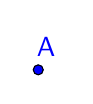
\begin{tikzpicture}[scale = 2]
	\draw
	(0,0) coordinate(A)
	(0.05,0.025) coordinate(pos)
	node[blue, anchor = south] {$\mathsf{A}$}  
	[blue,fill](A) circle(0.85pt); 
	\draw      [color = black](A) circle(0.9pt);
	\end{tikzpicture}
}
\newcommand{\Linustrik}{%  Strik, segment
	
\begin{tikzpicture}[scale = 0.4]
	\draw
	(0,0) coordinate(A)
	(1,0.7) coordinate(B)
	[line width = 1pt, blue](A)--(B);
	\draw[blue, fill](A) circle(4pt);
	\draw[blue, fill](B) circle(4pt);
	\end{tikzpicture}	
}

\newcommand{\Lina}{% bein lína, hægt að framlengja að vild
	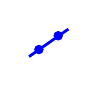
\begin{tikzpicture}[scale = 0.5]
	\draw
	(0,0) coordinate(A)
	(1,0.7) coordinate(B)
	[line width = 1pt, blue](A)--(B);
	\draw[blue, fill](0.25,0.18) circle(3pt);
	\draw[blue, fill](0.74,0.53) circle(3pt);
	\end{tikzpicture}	
}
\newcommand{\Halflina}{% við smíð á hornum
	
\begin{tikzpicture}[scale = 0.4]
	\draw
	(0,0) coordinate(A)
	(1,0.7) coordinate(B)
	[line width = 1pt, blue](A)--(B);
	\draw[blue, fill](A) circle(3pt);
	\draw[blue, fill](0.65,0.45) circle(3pt);
	\end{tikzpicture}	
	
}

\newcommand{\GeoO}{
	\begin{tikzpicture}[rotate=30,transform canvas={scale=0.18},yshift=7mm]
	\def\xrad{0.7}
	\def\yrad{0.58}
	\definecolor{GeogebraLitur}{rgb}{0.6,0.60,100}
	\tikzset{hnutur/.style={shape=circle, line width=0.7mm,color=black, fill=GeogebraLitur, scale=0.8, draw}} % 0.8
	\draw[ color = gray!70!black, line width=1.3mm] (0,0) circle[x radius = \xrad cm, y radius = \yrad cm];
	\def\n{5}
	\foreach \k in {1,...,\n}
	\node at ({360/\n*\k-10}:\xrad cm and \yrad cm)[hnutur] {};
	%	node[pos=1,hnutur]{} ;
	\end{tikzpicture}
}
\newcommand{\Geogebra}{{\color{gray!70!black}\textsf{Ge}\ \GeoO\textsf{Gebra }}}


%%%%%%%%%%%%%%%%%%%%%%%%%% Hyperlink References %%%%%%%%%%%%%%%%%%%%%%%%%%%
\usepackage{hyperref}

%--------------------% Storage Path for images %-----------------%
\graphicspath{{graphics/}{Graphics/}{./}}

\begin{document}
%Title of the report, name of coworkers and dates (of experiment and of report).
\begin{titlepage}
	\centering
	
\includegraphics[width=0.3\textwidth]{logopk.jpeg}\par\vspace{1cm}
	{\scshape\LARGE 
	Wydział Informatyki i Telekomunikacji
	\newline Analityka Danych
	\par}
	\vspace{1cm}
	{\scshape\Large Sprawozdanie z laboratorium 1\par}
	\vspace{1.5cm}
	{\huge\bfseries OpenMP\par}
	\vspace{2cm}
	{\Large\itshape Autorzy:}\par
	\vspace{2cm}
	{\Large\itshape Andrii Cherevko}\par
	\texttt{}\par

	{\Large\itshape Grzegorz Bogdał}\par
	\texttt{}\par
	\vfill
	Prowadzący:\par
	mgr inż. Wojciech Książek

	\vfill

% Bottom of the page
	{\large 13 października 2019\par}
\end{titlepage}

\section{Zbiór danych }
Wybrany przez nas zbiór danych to - Wine Quality Data Set
\url{(https://archive.ics.uci.edu/ml/datasets/Wine+Quality).}
 Zbiór miesci w sobie dane o jakości białego i czerwonego wina.
   Oryginalnie jest podzielony na 2 pliki : 
\begin{itemize}
  \item winequality-red.csv
  \item winequality-white.csv
\end{itemize}

W pierwszym pliku z próbkami czewonego wina znajduje się: 1600 próbek.
W drugim pliku z próbkami białego wina jest ich 4899.
Podczas wykonania pracy nad zbiorem stworzyliśmy plik train\_signals.csv
w którym są połączone cechy białego i czerwonego wina
oraz plik train\_labels.csv który zawiera w sobie klasy wina. Następnie losow wymieszaliśmy wiersze.

Oryginalny zbiór danych to próbki win portugalskich „Vinho Verde”.
Pojedyncza próbka jest opisana za pomocą 11 cech oraz oceny jakości wina (quality). Ocena jakości wina jest zmienną zależną. Cechy zapisane są w postaci
zmiennoprzecinkowej w pliku CSV.
Cechy opisujące wino to:
\begin{enumerate}
\item kwasowość stała
\item kwasowość lotna
\item poziom zawartości kwasu cytrynowego
\item zawartość cukru resztkowego
\item zawartość chlorków
\item zawartość wolnego ditlenku siarki
\item zawartość ditlenku siarki ogółem
\item gęstość
\item pH
\item poziom zawartości siarczanów
\item poziom zawartości alkohol
\end{enumerate}

\section{Parametry komputera}
Laboratorium zostało wykonane na komputerze o następującej konfiguracji:
\begin{table}[h]
    \centering
    \begin{tabular}{llr}
\hline

\cline{1-2}
Komponent   & Opis  \\
\hline
OS      & Arch Linux    \\

Kompilator      & gcc    \\

CPU      & AMD A10-6800K, 4 rdzenie fizyczne, brak hyperthreadingu    \\
          
RAM       & 16 GB 1866MHz DDR3           \\

\hline
\end{tabular}
\end{table}

\section{Metodologia}
W języku C++ zaimplementowano normalizację MinMax, standaryzację i algorytm knn dla k=1. Program zrównoleglono używając standardu OpenMP w kompilatorze gcc. Analogiczny program napisano w języku Python przy pomocy bibliotek pandas i sklearn. Następnie zmierzono czasy w zależności od liczby rdzeni dziesięciokrotnie i uśredniono zaprezentowane poniżej wyniki.

\pagebreak
\section{Wykres czasów normalizacji}

\begin{tikzpicture}[scale=1.5]
\begin{axis}[
title={Wykres czasów normalizacji MinMax - C++},
title style={text width=14em},
xlabel={Liczba wątków},
ylabel={Czas[s]},
xmin=0,xmax=4,
ymin=0,ymax=0.005,
legend pos=north west,
ymajorgrids=true,grid style=dashed
]

\addplot[color=red,mark=*]
coordinates {
(1, 0.000402915)
(2, 0.0010284)
(3, 0.00128433)
(4, 0.00104617)
};


\end{axis}
\end{tikzpicture}


\begin{tikzpicture}[scale=1.5]
\begin{axis}[
title={Wykres czasów normalizacji MinMax - Python},
title style={text width=14em},
xlabel={Liczba wątków},
ylabel={Czas[s]},
xmin=0,xmax=4,
ymin=0,ymax=0.005,
legend pos=north west,
ymajorgrids=true,grid style=dashed
]

\addplot[color=red,mark=*]
coordinates {
(1, 0.002195262908935547)
(2, 0.0021237850189208983)
(3, 0.0020517587661743166)
(4, 0.002150416374206543)
};


\end{axis}
\end{tikzpicture}

\begin{tikzpicture}[scale=1.5]
\begin{axis}[
title={Wykres czasów standaryzacji - C++},
title style={text width=14em},
xlabel={Liczba wątków},
ylabel={Czas[s]},
xmin=0,xmax=4,
ymin=0,ymax=0.005,
legend pos=north west,
ymajorgrids=true,grid style=dashed
]

\addplot[color=red,mark=*]
coordinates {
(1, 0.000284982)
(2, 0.000928761)
(3, 0.000921994)
(4, 0.00103475)
};


\end{axis}
\end{tikzpicture}

\begin{tikzpicture}[scale=1.5]
\begin{axis}[
title={Wykres czasów standaryzacji - Python},
title style={text width=14em},
xlabel={Liczba wątków},
ylabel={Czas[s]},
xmin=0,xmax=4,
ymin=0,ymax=0.005,
legend pos=north west,
ymajorgrids=true,grid style=dashed
]

\addplot[color=red,mark=*]
coordinates {
(1,0.003173565864562988)
(2,0.0031133651733398437)
(3,0.002929377555847168)
(4,0.003358006477355957)
};


\end{axis}
\end{tikzpicture}

\begin{tikzpicture}[scale=1.5]
\begin{axis}[
title={Wykres czasów KNN dla danych znormalizowanych metodą MinMax - C++},
title style={text width=14em},
xlabel={Liczba wątków},
ylabel={Czas[s]},
xmin=0,xmax=4,
ymin=0,ymax=0.3,
legend pos=north west,
ymajorgrids=true,grid style=dashed
]

\addplot[color=red,mark=*]
coordinates {
(1, 0.112567)
(2, 0.0627832)
(3, 0.0496401)
(4, 0.0338465)
};


\end{axis}
\end{tikzpicture}



\begin{tikzpicture}[scale=1.5]
\begin{axis}[
title={Wykres czasów KNN dla danych znormalizowanych metodą MinMax - Python},
title style={text width=14em},
xlabel={Liczba wątków},
ylabel={Czas[s]},
xmin=0,xmax=4,
ymin=0,ymax=0.3,
legend pos=north west,
ymajorgrids=true,grid style=dashed
]

\addplot[color=red,mark=*]
coordinates {
(1, 0.14634275436401367)
(2, 0.2372218608856201)
(3, 0.19606773853302)
(4, 0.20869193077087403)
};


\end{axis}
\end{tikzpicture}



\begin{tikzpicture}[scale=1.5]
\begin{axis}[
title={Wykres czasów KNN dla danych standaryzowanych - C++},
title style={text width=14em},
xlabel={Liczba wątków},
ylabel={Czas[s]},
xmin=0,xmax=4,
ymin=0,ymax=1,
legend pos=north west,
ymajorgrids=true,grid style=dashed
]

\addplot[color=red,mark=*]
coordinates {
(1, 0.896477)
(2, 0.461227)
(3, 0.376144)
(4, 0.267142)
};


\end{axis}
\end{tikzpicture}




\begin{tikzpicture}[scale=1.5]
\begin{axis}[
title={Wykres czasów KNN dla danych standaryzowanych - Python},
title style={text width=14em},
xlabel={Liczba wątków},
ylabel={Czas[s]},
xmin=0,xmax=4,
ymin=0,ymax=1,
legend pos=north west,
ymajorgrids=true,grid style=dashed
]

\addplot[color=red,mark=*]
coordinates {
(1, 0.1461501121520996)
(2, 0.2383200168609619)
(3, 0.18554110527038575)
(4, 0.20907130241394042)
};


\end{axis}
\end{tikzpicture}

\textbf{\textit{Uwaga:}} Wykresy bazują się na średniej z czasów dla każdej z metod z 10 powtórzeń









\section{Podsumowanie}

Biblioteka sklearn nie oferuje opcji zrównoleglenia normalizacji i standaryzacji. Implementacja w języku C++ staje się wolniejsza wraz z liczbą wątków. Implementacja autorów w języku C++ jest szybsza. Przypuszczalnie z uwagi na szybką implementację i mały zbiór danych narzut związany z utworzeniem wielu wątków neguje korzyści związane z równoległości, które uwidoczniłyby się na większym zbiorze.

W przypadku zrównoleglenia algorytmu kNN w języku C++ można zobaczyć znaczne przyspieszenie czasów przy zwiększeniu ilości wątków. W implementacji autorów wszystkie wątki przeszukują jeden zbiór danych bez kopiowania go, przez co narzut związany z równoległością jest minimalny. Dla danych znormalizowanych metodą MinMax implementacja autorów jest szybsza od implementacji biblioteki sklearn. 
W przypadku implementacji kNN w Python zrównoleglenie spowalnia wykonanie programu. Czas wzrasta gdy pojawia się drugi wątek, kolejne wydają się nie mieć wpływu. Autorzy sprawozdania nie rozumieją tego zachowania.



\bibliographystyle{IEEEtran}
\bibliography{references}


%------ To create Appendix with additional stuff -------%
%\newpage
%\appendix
%\section{Appendix/Fylgi gögn}
%Put data files, CAD drawings, additional sketches, etc.

\end{document}
